\chapter{Cadyts}
\label{ch:cadyts}
% ##################################################################################################################

\hfill \textbf{Authors:} Kai Nagel, Michael Zilske, Gunnar wo?

\begin{center} 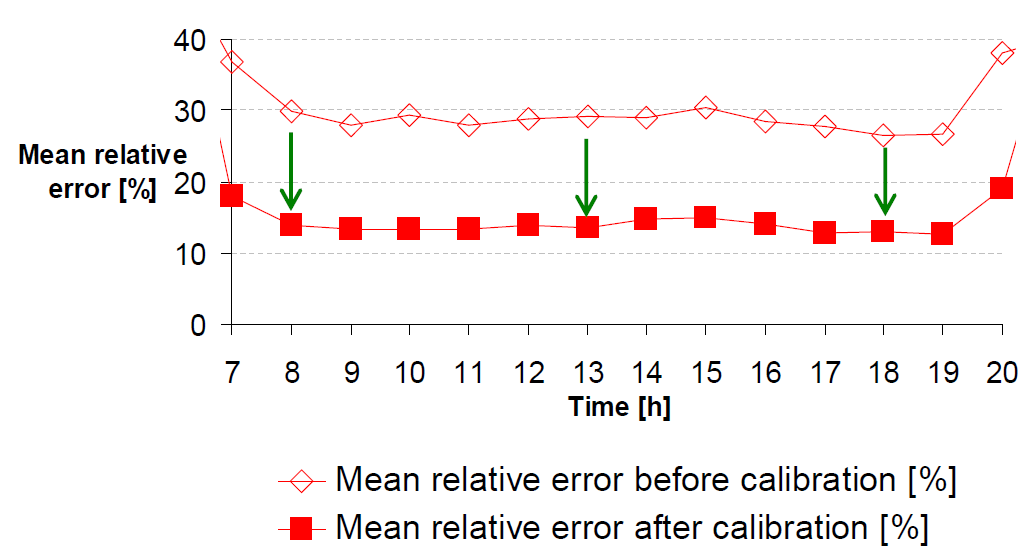
\includegraphics[width=0.4\textwidth, angle=0]{extending/figures/cadyts/cadyts} \end{center}

\createStandardInformation{cadytsIntegration}{\lstinline{RunCadyts4CarExample} class}{cadytsCar}{\citet[][]{cadyts-manual, floetteroed-2010e, FloetteroedChenEtAl2011BehavioralCalibAndAnaNETS, Floetteroed2008PhD, Moyo2013PhD,FloetteroedBierlaireNagel2010Bayesian}}

% ##################################################################################################################

\ah{adopted from \citet[][]{Floetteroed2009CadytsSTRC}. Please check, in particular copy rights of figure}

% ##################################################################################################################
\section{Introduction}
\gls{cadyts}\footnote{\url{http://people.kth.se/~gunnarfl/cadyts.html}}---licensed under \gls{gplv3}---estimates, \ie calibrates, disaggregate demand models of \gls{dta} simulators from traffic counts and vehicle re-identification data. \gls{cadyts} is compatible with a broad class of \gls{dta} microsimulators, and can be be hooked into simulators by sparse interfaces.

As explicated in formal terms in Chapter~\ref{ch:abta} and~\ref{ch:montecarlo}, \gls{dta} targets at consistency between a dynamic model of travel demand---in \gls{matsim} represented by the agents' plans---and a dynamic model of network supply, \ie traffic flow dynamics. 

\gls{cadyts} improves on the method by adjusting the plan choice probabilities of all agents such that they result in simulated network conditions that are consistent with measured real-world data, often traffic count data. Adjustment of plan choice probability is naturally done by adjusting the plans utility as shown in the next section.

% ##################################################################################################################
\section{Adjusting Plans Utility}
In case of count data being the empirical source, the plan-specific utility corrections are composed of link- and time-additive correction terms $\Delta V_a(k)$. 
In case congestion is light and traffic counts are independently and normally distributed, these link- and time-additive correction terms become \cite[p.487]{FloetteroedChenEtAl2011BehavioralCalibAndAnaNETS}
%
\begin{equation}
\Delta V_a(k) = \frac{y_a(k) - q_a(k)} {\sigma_a^2(k)} \ ,
\label{eq:cadyts:correction}
\end{equation}
%
where $y_a(k)$ is the real-world traffic, $q_a(k)$ is the simulated traffic count, and $\sigma^2_a(k)$ is the variance of the traffic count at location $a$ for time bin $k$.
%
%(its calculation is for example explained by \citet[p.54]{Moyo2013PhD} \kai{das ist eigentlich auch keine gute Referenz dafür; gibt es nicht etwas von Gunnar selber?  (Aber das enthält einen Fehler, oder wie war das?)}).
%\dominik{Bei Manuel stand bzgl. des sigma einfach etwas mehr, deswegen war er hier die Referenz}

The utility correction of a given activity-travel plan of an agent is calculated as the sum of all $\Delta V_a(k)$ that are covered by the plan \citep{FloetteroedChenEtAl2011BehavioralCalibAndAnaNETS}. 
With this, the \textit{a posteriori} choice probability of plan $i$ of agent $n$ becomes
%
\begin{equation}
P_n(i|\vec{y}) \sim \exp\left(V_n(i)+ \sum_{ak\in_{}i}   \frac{y_a(k)-q_a(k)}{\sigma^2_a(k)} \right)	
\label{eq:cadyts:selection}
\end{equation}
where $V_n(i)$ is the \textit{a priori} score of a plan $i$ of agent $n$ as calculated for example with Equation~(\ref{eq:matsimUTF}).
%The notation $ak \in i$ means all links $a$ and time slots $k$ in which the plan $i$ influences the measurements on those links.
%
Intuitively, if the simulation value, $q_a(k)$, is smaller than the measurement from reality, $y_a(k)$, an increase in score and thus an increase in choice probability results. 
$\sigma_a(k)$ denotes how much one should trust that specific measurement---a large $\sigma_a(k)$ implying a large variance and thus a low trust level.

%% \begin{equation}
%% = P_n(i) \cdot \exp\left( \sum_{ak\in_{}i}   \frac{(y_a(k)-q_a(k))}{\sigma^2_a(k)} \right)	
%% \end{equation}

%% $P_n(i)$ is the \textit{a priori} choice probability of plan $i$ of agent $n$, and 

% ##################################################################################################################
\section{Hooking Cadyts Into MATSim}
Hooking \gls{cadyts} into \gls{matsim} requires following operations:
\begin{enumerate}
\item Initialization: When the calibration is started, it needs to be provided with all available traffic counts and some further parameters.
\item Iterations: The calibration is run jointly with the simulation until (calibrated) stationary conditions are reached.
	\begin{compactitem}[(a)]
	\item Demand simulation: The calibration needs an access point in the simulation in order to affect the plan choice. There are various ways to realize this, depending on the concrete simulator.
	\item Supply simulation: The calibration needs to observe the simulated network conditions in order to evaluate their deviation from the traffic counts.
	\end{compactitem}
\end{enumerate}

\gls{matsim} implements these operations as follows.

\begin{enumerate}
\item Initialization: The function \lstinline|void addMeasurement(...)| is called once for every measurement before the simulation starts. It registers a measurement of a certain type, which has been observed on a certain link.
%
\item Iterations:
	\begin{compactitem}[(a)]
	\item Demand simulation: Whenever an agent chooses a plan, he or she asks the calibration through the function \lstinline|boolean getSampler(Object agent).isAccepted(Plan<L> plan)| if the plan is accepted or if another plan needs to be generated.
%
	\item Supply simulation: The function \lstinline|void afterNetworkLoading(SimResults<L> simResults)| is called once after each network loading. It passes a container object to the calibration that provides information about the results of the most recent network loading, in
particular about the simulated flows at the measurement locations.
	\end{compactitem}
\end{enumerate}

% ##################################################################################################################
\section{Applications}
\gls{cadyts} has been successfully applied in studies such as \citet[][]{ZiemkeNagelBhat2014IntegratingCemdapMatsimTransferabilityVSPWP, ZilskeNagelPhoneTracesAndCadyts, FloetteroedEtAl2009IatbrCalibration, FloetteroedChenEtAl2011BehavioralCalibAndAna}. 
Its efficiency is evident in the Zürich scenario results as shown in \citet[][Slide~8]{FloetteroedEtAl_unpub_MATSimUserMeeting_2011}, reproduced in Figure~\ref{fig:cadyts}.

\createfigure%
{Zürich case study results: mean relative error in link volumes}%
{Zürich case study results: mean relative error in link volumes \ah{get printable version}}%
{\label{fig:cadyts}}%
{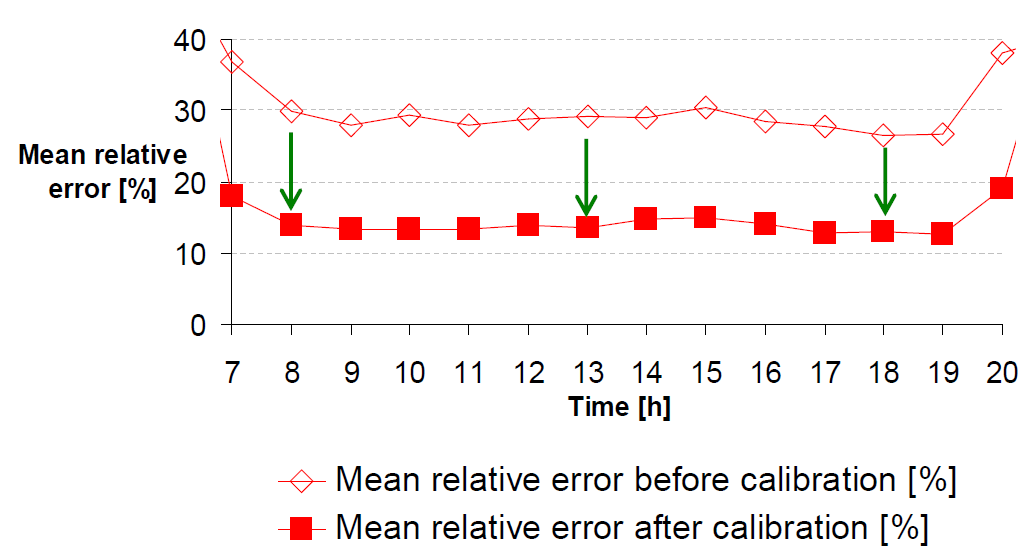
\includegraphics[width=0.8\textwidth, angle=0]{extending/figures/cadyts/cadyts}}%
{\citet[][Slide~8]{FloetteroedEtAl_unpub_MATSimUserMeeting_2011}}

% ##################################################################################################################
% Local Variables:
% mode: latex
% mode: reftex
% mode: visual-line
% TeX-master: "../../main"
% comment-padding: 1
% fill-column: 9999
% End: 
